
%dash pattern=on 5pt off 2pt
%[fill = white, rounded corners = 5pt, inner sep=0.8pt]
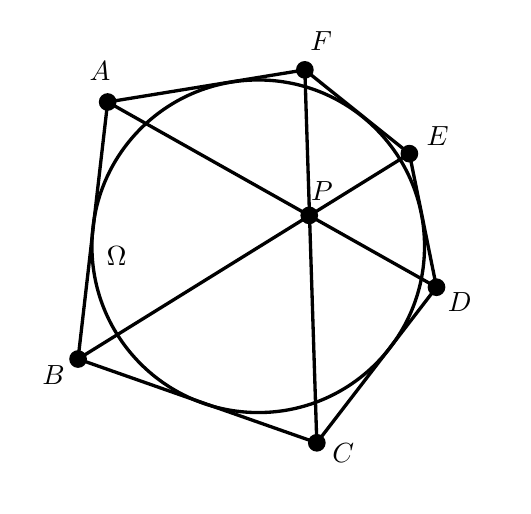
\begin{tikzpicture}[scale = 0.8]
    \clip(-3.31,-2.66) rectangle (4.24,4.62);
    \draw [line width=1.2pt] (0.35,1.15) circle (2.64cm);
    \draw [line width=1.2pt] (-2.04,3.44)-- (-2.51,-0.64);
    \draw [line width=1.2pt] (-2.51,-0.64)-- (1.28,-1.97);
    \draw [line width=1.2pt] (1.28,-1.97)-- (3.18,0.5);
    \draw [line width=1.2pt] (3.18,0.5)-- (2.75,2.62);
    \draw [line width=1.2pt] (2.75,2.62)-- (1.09,3.95);
    \draw [line width=1.2pt] (1.09,3.95)-- (-2.04,3.44);
    \draw [line width=1.2pt] (-2.04,3.44)-- (3.18,0.5);
    \draw [line width=1.2pt] (1.09,3.95)-- (1.28,-1.97);
    \draw [line width=1.2pt] (2.75,2.62)-- (-2.51,-0.64);
    \begin{scriptsize}
        \normalsize
        \draw[color=black] (-1.9,1)node {$\Omega$};
        \fill [color=black] (-2.04,3.44) circle (4.0pt);
        \draw[color=black] (-2.16,3.93) node {$A$};
        \fill [color=black] (-2.51,-0.64) circle (4.0pt);
        \draw[color=black] (-2.9,-0.9) node {$B$};
        \fill [color=black] (1.28,-1.97) circle (4.0pt);
        \draw[color=black] (1.7,-2.14) node {$C$};
        \fill [color=black] (3.18,0.5) circle (4.0pt);
        \draw[color=black] (3.55,0.27) node {$D$};
        \fill [color=black] (2.75,2.62) circle (4.0pt);
        \draw[color=black] (3.2,2.9) node {$E$};
        \fill [color=black] (1.09,3.95) circle (4.0pt);
        \draw[color=black] (1.35,4.4) node {$F$};
        \fill [color=black] (1.16,1.64) circle (4.0pt);
        \draw[color=black] (1.36,2.02) node {$P$};
    \end{scriptsize}
\end{tikzpicture}